\chapter{绪论}
 % 简短的介绍
 关系市场营销是指企业为了建立和维护企业与顾客之间、企业与渠道商之间的长期关系,所产生的一系列营销决策过程。该过程的最终目的是最大化企业的长期收益,科学的开展关系市场营销对企业的生存和发展起到重要作用。强化学习是一类机器学习方法,也用于解决序贯决策问题,并且其累计奖赏最大化的目标与关系市场营销中的长期收益最大化的目标不谋而合,所以使用强化学习技术解决关系市场营销问题有着其它机器学习技术无法比拟的优势。

\section{研究背景及意义}

 % 1、市场营销的背景、含义和意义、进而引出直效营销和广告投放
 % 2、强化学习的出现的背景以及为什么可以用于解决CRM问题,但是解决这个问题还有什么问题。

在中国改革开放和国际化进程的不断深入下,全社会对市场、对营销、对管理的态度发生了从无知到有知,从漠视到重视的巨大转变。时至今日,我们发现我们好像从来没有与世界的脉搏如此的接近过,同样,我们的企业和国家也从来没有如此深切的感受到全球化的竞争是如此的残酷。因为市场竞争的不断加剧,每个企业都在努力寻找着自己的核心竞争能力,以期望能在激烈的竞争中取得优势。但是,近年来,随着信息技术的广泛使用,众多行业的产品在价格、质量和服务上的差异越来越小,如何在如此激烈的市场竞争中领先对手,给当前的商业研究提出了新的要求,市场营销就是其中一个重要的研究方向。

美国著名营销学者菲利普$\cdot$科特勒在《营销管理》\citep{菲利普2016营销管理}这一被世人誉为营销学圣经的书中指出:市场营销是个人或群体通过创造、提供并同他人交换有价值的产品,以满足各自需求和欲望的一种社会活动和管理。中国学者谭思敏在其书\citep{谭思敏2008中国式营销}中对这一定义进行了深刻分析,并强调:在市场营销过程中,企业应该在对市场中各方关系进行充分分析的基础上,以市场需求为导向,规划全部经营活动,以保持企业与各方的长期良好关系,才能最大化企业的长远利益。这就是关系企业营销,它包括企业与顾客、渠道商、政府机构等之间的关系,本文主要关注前两个方面,即客户关系管理和渠道关系管理。

关系市场营销所涉及的研究内容非常广泛,研究方向也朝着多元化的趋势发展\citep{王广宇2013客户关系管理}。在过去的二十年里,随着互联网和数据库的广泛应用,各个行业、各个公司每天都会积累一定的商业数据,如何将这些原始数据进行实时和更深层次的分析,以辅助或代替企业进行商业决策,成为近年来关系市场营销中最为活跃的研究内容。其中,最有代表性的方向是将市场营销与机器学习技术的融合,利用机器学习技术从营销数据中提取出其背后的关系信息,然后利用这些信息进行预测、分析和决策,以达到最大化企业收益的目的。



本文分别关注于客户关系管理中的直效营销场景和渠道关系管理中的广告渠道预算分配场景,并着眼于基于值函数的强化学习模型在解决以上两个场景时存在的问题,提出相应的改进模型。现对以上两个场景进行介绍。

1)直效营销(Direct Marketing,DM)场景。直效营销是客户关系管理中的典型应用,它强调与客户建立长期的关系,以达到最大化顾客的生命周期价值的目的。在该营销过程中,企业需要根据提前收集到的顾客资料和其消费历史记录等信息,构建关于顾客未来是否会发生购买行为的响应模型,应用到真实的营销活动中,以提高顾客的响应概率,最大化企业的长期收益。需要强调的是:直效营销特指不通过第三方,中间人,而直接对客户进行营销的方式,所以企业也会直接得到每一位顾客的反馈信息,具体过程如图$\ref{fig:直效营销示意图}$所示。
\begin{figure}[htbp]
\centering
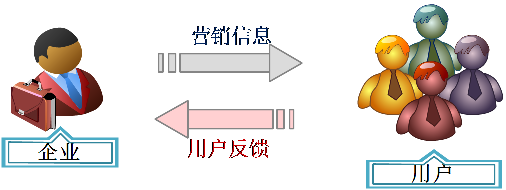
\includegraphics[width=0.5\textwidth]{直效营销示意图}
\caption{直效营销场景示意图}
\label{fig:直效营销示意图}
\end{figure}

2)多渠道广告预算分配(Budget Allocation among Multi-Channel Advertising ,BAMCA)场景。在现在的商业社会中,如果单单根据企业自己获取的顾客信息进行直效营销,其效率和速度是非常慢的,已经无法满足当下激烈而残酷的商业竞争环境了。所以,出现了很多拥有众多优质广告渠道资源的广告代理机构(Ad-Agence),他们拥有大量而丰富的客户资源,可以帮助企业进行更深入、更广泛的营销推广。(为了书写方便起见,后文中将多渠道广告预算分配问题简称为广告预算分配问题,或者BAMCA问题)

需求方平台(Demand-Side Platform,DSP)是一种新型在线广告代理平台,起源于美国。它服务于广告主,帮助广告主在互联网或者移动互联网上进行广告投放,DSP可以使广告主更简单、更便捷地遵循统一的竞价和反馈方式,对位于多家广告交易平台(Ad Exchange)的在线广告,以合理的价格实时购买高质量的广告库存。DSP让广告主可以通过一个统一的接口来管理一个或者多个Ad Exchange账号,甚至DSP可以帮助广告主直接管理Ad Exchange的账号,提供全方位、自动化的服务。简单来说,在DSP上有充足的渠道资源和统一的竞价策略,所以广告主只需要关注两个问题:选择什么样的投放渠道,进行多少金额的投放花费,即投放策略的制定,然后,DSP就会按照广告主的投放策略进行投放(购买广告位),投放结束后,再将投放效果信息反馈给广告主。如图$\ref{fig:广告渠道预算分配示意图}$所示为基于DSP的广告投放示意图。
\begin{figure}[htbp]
\centering
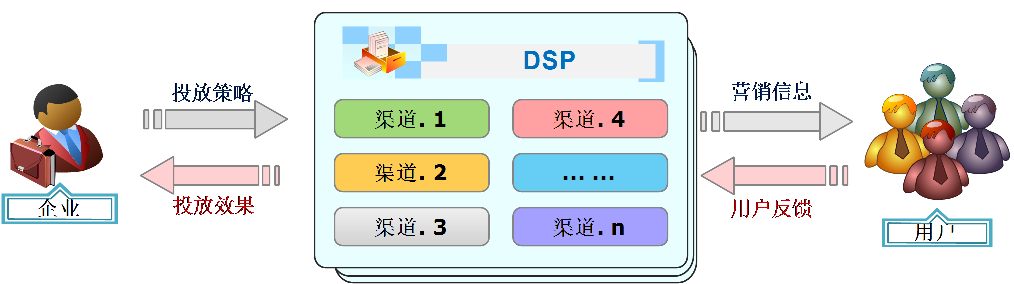
\includegraphics[width=0.9\textwidth]{投放渠道预算分配示意图}
\caption{基于DSP的广告投放示意图}
\label{fig:广告渠道预算分配示意图}
\end{figure}

在企业使用DSP进行实际营销时,为了达到更有效、更充分的的投放效果,一般会选择多个渠道进行长时间的持续投放。另外,为了财务帐面的稳定,企业会提前给出每一天的广告投放预算,然后营销人员需要制定有效的投放策略,将预算合理的分配给多个渠道,以使的企业产生的整体收益最大化,这就是本文的所研究的广告渠道的预算分配的场景。

通过对直效营销场景的研究,可以帮助企业在处理好与用户之间的关系的基础上,最大化用户的生命周期价值。通过对投放渠道预算分配问题的研究,可以帮助企业在处理好与营销渠道之间的关系的基础上,最大化多渠道的整体长期收益。另外,
% 经过稍微的修改,
还可以将以上两个场景的研究成果拓展到其它的应用场景中,比如广告精细化推荐、点击率预估等问题,以辅助企业做出智能化的营销决策。总之,研究关系企业营销,可以提升企业关系的管理水平、树立企业新型营销理念、降低企业成本、提高企业效益,进而全面提高企业的核心竞争力,因此针对关系市场营销的研究具有重要的研究前景和商业价值,同时,针对强化学习的研究和改进并将拓宽其它应用领域,对强化学习的发展也有着重要而深远的意义。

\section{国内外研究现状}
因为本文的研究思路是从基于值函数的强化学习模型出发,着眼于模型在以上两个场景的应用中存在的问题,提出相应的改进模型。所以该部分将关系市场营销和强化学习的研究现状进行分别介绍。

\subsection{关系市场营销的研究现状}
关系市场营销最早是由德克萨斯大学的林·贝利提出,其主要是针对客户关系管理的研究,但是哈佛大学的西奥多·利维特最早将营销的范围进行了拓宽,提出了针对其它关系市场营销方面的研究,之后的众多学者在供应商、分销商等渠道关系管理上进行了大量的研究。本文主要关注客户关系管理中的直效营销场景以及渠道关系管理中的基于DSP的广告渠道预算分配场景,其中,目前针对后一个应用场景的相关研究较少。本节主要将关于机器学习在这两个场景中的研究现状进行介绍。

% 虽然CRM一词最早出现在1999年,但是相关理论的研究已有百余年之久。总的来看CRM大概经历了CRM理念萌芽时期、CRM应用雏形化时期、CRM产品实用化时期以及CRM智能化集成时期\citep{王广宇2013客户关系管理},其中,CRM智能化集成就是指将人工智能等手段集成到CRM应用中,多年来,经过众多学者和专家的不断努力,已经在此方面取得了瞩目的成果\citep{bahari2015efficient,farquad2014churn,linoff2011data,chiang2018applying,ballings2015crm},并将其应用到各种商用CRM系统中,比如国外微软公司的Dynamics CRM、甲骨文公司的Siebel、People Soft以及惠普公司的Front Office等CRM产品,国内主要有用友公司的TruboCRM产品,立有信公司的MyCRM产品等。由于本文主要关注直复营销活动和多渠道广告投放两个应用场景,因此主要将这两个方面的研究现状进行详细介绍。

\paragraph{直效营销}
直效营销最早可以追溯到十九世纪六十年代,也是最早、最经典营销形式之一,之后的大部分营销模型都是在此基础上发展而来的。但是,数十年来,众多学者主要是将监督和非监督的机器学习方法应用到直效营销问题的研究上。

1975年Stone出版的《successful direct marketing methods》\citep{stone1988successful}一书,第一次系统的介绍直效营销的各种应用场景、概念以及特点等,为后续直效营销的研究打下了坚实的基础。2005年,Wong等人\citep{wong2005mining}针对直效营销场景中顾客购买的可能性与购买所花费的金额之间往往会呈现一定的负相关性这一问题,提出直接估计客户产生的利润而不是估计客户购买的概率的思想,进而使用关联规则的方法用于构建预测未来客户价值的模型,使用KDD-CUP-98作为数据集进行测试,取得了比该比赛的冠军高出了41%利润率的效果。2013年Coussement等人\citep{coussement2015improving}较为细致和全面的介绍了大部分的数据挖掘技术(逻辑回归、线性二次判别分析法、朴素贝叶斯、神经网络、决策树以及KNN算法)在四个直效数据集上的应用情况,并且通过权衡结果的可解释行和准确性之间的关系,给出了如何进行算法选择的建议。通过实验发现,CHAID,CART和神经网络算法在测试集上的表现要好于其他的算法。需要特别提到的是,在文献\citep{ngai2009application}中,作者详细总结了客户关系管理领域的近千篇文章,其中涵盖了客户关系管理的四个不同的场景以及数据挖掘的七种技术算法,研究结果表明,分类和关联模型是数据挖掘技术在客户关系管理领域中最常用的两类模型。

% 文献。文献\citep{karim2013decision}将朴素贝叶斯算法和C4.5决策树算法分别应用到银行的直销推广活动中,以此来预测客户是否会订购定期的理财产品,然后使用一个新的算法\citep{alam2012actionable}从预测结果中提出可行的营销行为知识,并在UCI公开数据集上对这两种算法的性能进行了对比,得出C4.5决策树算法在预测的准确度(Accuracy)、ROC值、精确度(Precision)等方面都好于朴素贝叶斯算法的结论。文献

% 文献\citep{parlar2017using}主要关注是的是特征选择,使用信息增益和卡方的方法来选择重要的特征,然后使用朴素贝叶斯算法来比较这两个特征选择的方法,实验表明,提出的方法在减少特征集的同时提高的分类性能。

% 国内关于直复营销的研究起步相对较晚,研究人员也相对较少,大多集中于营销理论的研究,而对基于机器学习技术的直复营销策略的研究相对较少。但是,近年来经过学者们的不断努力,在相关领域也取得了很多实质性的进展。文献\citep{徐笑昂2007直复营销模式下的商品选择和顾客分群算法研究}针对商品选择和顾客之间的密切关系,提出了一种顾客导向下基于交叉营销的双重分割算法DualSeg,主要适用关联规则挖掘商品与商品之间、顾客与顾客之间以及顾客与商品之间的影响,从而解决了直复营销中的商品选择和顾客分群问题。文献\citep{chen2015behavior}针对营销中存在异构型数据的特点,提出了一种改进的分层多核支持向量机模型(H-MK-SVM)用于感知用户的响应模型,该模型可以从众多异构数据中进行数据转换和特征提取,将异构高维多关系型的数据转换为以客户为中心的高阶张量型数据进而可以提取特征属性,通过使用真实的营销数据验证了该改进模型比其他模型(SVM、Adaboost等)在准确度上的优越性。文献\citep{sing2013data}提供了一个基于机器学习技术在直邮营销方面的通用框架,详细描述了框架中的各个流程,最后通过实验评估,证明了该框架降低降低时间开销的同时较少了企业的营销成本。

通过对上述文献的研究成果进行分析,可以发现:在基于监督学习和非监督学习的方法中,主要是预测用户在下一时间点是否会发生购买行为或者发生的购买行为的概率,进而得出在下一时间点应该做出什么样的营销方案,可以使的企业所获的的当前收益最大化。但是,这种方法存在以下不足:

1)在监督学习中,存在前提假设是数据已经对环境进行了充分的探索,然后从给定的带标签的样本中拟合模型。但是,如果样本中本来就没有最优的营销行为,那么监督学习是永远都无法学习到最优的营销方案的。

2)基于监督学习和非监督学习的模型只考虑了当前时刻的即时利润(Immediate Profits)最大化,而忽视长远利润,不符合企业营销的最终目标。因为,即使在这一时刻做出了目前看来是最优的营销方案,但是该方案可能会对之后的营销方案产生潜在的负面的影响,从而影响了整体的利润最大化。

% 即采取什么样的营销行为,可以使的这一次营销的利润最大化,这样就仅仅考虑了即时利润,

而强化学习可以通过在训练时引入探索的方式以及将累积奖赏最大化作为优化目标来解决以上两个问题。因此,近年来有学者开始使用强化学习来解决直效营销问题。

2002年,Pednault等人\citep{pednault2002sequential}首次将强化学习技术用于解决直效营销问题,提出使用批Q-learning(Batch Q-learning)的方法对该场景进行建模,进而进行策略的学习与优化,最后通过基于KDD-CUP-98数据集的仿真实验表明,该模型在连续营销的长期收益上高于其它的模型。2013年,Silver等人\citep{silver2013concurrent}提出了一种基于时间差分学习的并行强化学习框架。通过该框架可以并发的实现企业与客户之间的交互,并且通过模拟器分别在非自举(Non-bootstrappig)、非在线(Non-online)和非序列化(Non-sequential)三个方面进行了模型的对比评估,得到了在高并发的序列化问题中,应该考虑使用进行自举、在线学习以及使用序列化的强化学习方法的结论。2015年Tkachenko等人\citep{tkachenko2015autonomous}使用了深度强化学习解决直效营销中的问题,即使用Q-learning的方法训练一个深度神经网络来学习客户的状态和营销行为之间的关系,同时,该文章使用Recency-Frequency-Monetary指标参数化客户状态空间,实现了顾客响应率和顾客花费金额两方面的显著提高。

\paragraph{广告渠道预算分配}
广告渠道预算分配是属于资金分配问题,是经济学、运筹学和管理科学等领域中的一个经典问题\citep{zhang2017multi}。与直效营销应用场景的目标相同,广告渠道预算分配问题也是为了追求长期收益最大化。

2012年Yang等人\citep{yang2012budget}针对搜索广告资金分配的优化问题,提出了一个分层的预算分配优化框架,通过该框架可以实现广告预算的分配
和实时调整,其中位于第二层的活动层(Campaign Level),主要是用于解决预算在多个渠道中的分配问题,经过评估实验验证了此框架产生的策略优于实际广告中常用的两种基准投放策略。2013年Ding等人\citep{ding2013multi}研究了带有预算约束的多臂老虎机问题(Multi-Armed Bandit Problem, MAB),提出了基于置信区间上界的改进方法,理论证明了该算法的后悔界(Regret Bound)为$O(lnB)$(其中$B$代表预算金额),具有很好的学习能力,最后通过真实的广告投放,验证了算法的有效性。2016年Boutilier等人\citep{boutilier2016budget}提出带预算约束的MDPs(BMDPs)算法,通过权衡预算分配和期望收益之间的关系得到一个关于预算的函数,并证明该函数是非递减的凹函数,然后通过动态规划的方法求出该问题的解。2017年Zhang等人\citep{zhang2017multi}提出将多渠道广告投放资金问题转化为权重未知的多选择背包问题(Multi-Choice Knapsack Problem, MCKP),然后又提出了两种权重阈值的搜索方法,从理论和仿真实验两方面都证明了该搜索方法的有效性。

但是,基于DSP的广告渠道资金分配问题并没有得到关注,而且因为不同场景存在不同的特点,也无法直接将上述模型直接应用于该场景中。

\subsection{强化学习的研究现状}
% 介绍强化学习的发展、热点和未来发展趋势
此部分将分为强化学习的总体发展历程、研究热点以及强化学习的发展趋势等三个方面进行展开介绍。

\paragraph{发展阶段}
强化学习的发展过程大概可以分为三个阶段。

第一阶段是1998年以前,这一阶段形成了强化学习基本理论框架,学者们关注和发展的最多的算法是基于表格型的强化学习算法,包括值迭代和策略迭代。代表性的工作是强化学习鼻祖Richard将其专刊装订成书,这标志着强化学习发展成为机器学习领域的一个重要分支。该书《Reinforcement Learning: An introdcution》是强化学习领域的经典著作,第一次系统而全面的介绍了强化学习的相关理论知识,至今仍然被广大的教育机构和强化学习爱好者作为强化学习的经典教材(该书最新电子版可在网上免费获取\footnote{http://incompleteideas.net/book/bookdraft2017nov5.pdf}),需要注意的是,这期间还出现了强化学习代表性算法Q-learning\citep{watkins1992q}和Sarsa\citep{rummery1994line}。

第二阶段是1998年到2013年,这一阶段基于直接策略搜索的强化学习方法得到了深入研究和发展。自从Williams在其论文\citep{williams1992simple}中提出直接对Reinforce算法的策略梯度进行估计这一方法后,出现了各种改进方法,如:GPOMDP\citep{baxter2001infinite}、PEGASUS\citep{neumann2005reinforcement}以及与值函数结合的Actor-Critic算法\citep{konda2000actor}等。

第三阶段是2013年以后,随着深度学习的发展,这一阶段出现了深度强化学习算法。代表性的工作是DeepMind团队提出了DQN(Deep Q Network)算法并将其成功应用在雅达利(Atari)游戏中\citep{mnih2013playing},之后无数的学者对其进行了改进研究,但是
大部分都应用在机器人和游戏中。
其中,最具轰动性的事件当属在2016年和2017年,谷歌的AlphaGo利用深度强化学习算法连续两年分别击败了世界围棋冠军李世石和柯洁。

\paragraph{研究热点}
但是,目前强化学习在实际应用中仍然存在维度灾、收敛速度慢等问题,其中维度灾是指在大空间和连续问题中,强化学习无法在有限的空间和时间内学习到一个合理的解决方案,而收敛速度慢又与强维度灾有着密切的关联,所以解决维度灾问题对强化学习的应用起到了十分重要的作用。近年来,众多研究者主要集中于利用函数逼近的方法解决此问题,而函数逼近方法又可以分为参数化函数逼近方法和非参数化函数逼近方法。

参数化函数逼近方法又可以分为线性函数逼近和非线性函数逼近两种方法。其中在线性函数逼近中,基函数的形式和参数个数需要提前制定,往往会限制函数的逼近能力。该方法最早是由Samuel在1967年提出,并将其应用于西洋跳棋的系统设计中\citep{samuel1959some}。1988年,Sutton提出将线性函数逼近法与带有资格迹的时间差分(Temporal Difference, TD)方法相结合,然后使用梯度下降求解近似值函数的方法后\citep{sutton1988learning},掀起了线性函数逼近法研究的热潮,相继出现了最小二乘时间差分(Least Squares Temporal Difference, LSTD)算法\citep{bradtke1996linear}、离策略(Off-policy)函数逼近方法\citep{precup2001off}、以及梯度时间差分(Gradient Temporal Difference, GTD)学习算法\citep{sutton2009convergent}等,其中GTD解决了离策略TD学习算法的不稳定问题,且具有较低的时间负责度\citep{sutton2009convergent}。

非线性函数逼近方法中的函数逼近器是关于参数的非线性函数,如神经网络。虽然该方法具有很强的表征能力,但是容易陷入局部最优,且收敛性难以保证。1995年Bertsekas等\citep{bertsekas1995neuro}利用前向神经网络逼近强化学习中的值函数,取得了相比线性逼近较好的结果,但是往往会出现不稳定不收敛的情况。直到DeepMind团队于2013年提出了DQN网络,才使的这一问题得到有效解决。在DQN网络中,通过在训练过程进行经验回放\citep{mnih2013playing}和单独设立目标网络\citep{mnih2015human}这两种改进方法,打破了数据之间的关联性,使的神经网络的训练过程收敛且稳定,并且在游戏中取得了令人振奋的表现。从此以后,彻底掀起了学术界和工业界研究深度强化学习的热情。2015年DeepMind团队又提出了Double DQN模型,在该模型中为了克服Q-learning本身固有的缺点——过估计(Overestimate),将动作的选择和动作的评估分别使用不同的值函数来实现。除此以外,深度Sarsa、A3C(Asynchronous Advantage Actor-Critic)、DDPG(Deep Deterministic Policy Gradient)等一些列有影响力深度强化学习模型相继被提出。

非参数化函数逼近法,并不是没有任何参数的函数逼近,而是指参数个数和基函数的形式并非固定,完全由样本决定,因此具有更大的灵活性和表征能力,但是当样本量很大时,将会带来更大的计算开销。非参数化函数逼近模型主要有基于高斯过程和基于核方法的值函数逼近模型。其中,基于核方法的研究相对较多,如基于核的强化学习函数逼近方法\citep{ormoneit2002kernel}、基于核的最小二乘TD方法(Kernel-based Least Squares TD, KLSTD)\citep{xu2005kernel}、基于最小二乘的策略迭代算法等(Kenel-based Least Squares Policy Iteration, KLSPI)\citep{xu2007kernel}等。

\paragraph{发展趋势}
强化学习正在飞速发展,从当前的论文中可以初步判断强化学习的发展具有如下趋势:1)强化学习与深度学习的结合会更加紧密。2)强化学习与领域知识的结合更加紧密,特别是在重塑回报函数的方向上。3)强化学习的理论分析会更加全面、具体,算法性能会更加稳定和高效。本文所提出的改进模型属于前两点。

\section{主要研究内容}
如图$\ref{fig:研究内容}$所示,本文从基于值函数逼近的强化学习模型出发,着眼于模型在直效营销(客户关系管理)和广告渠道预算分配(渠道关系管理)中存在的问题,提出相应的改进方法,最后通过仿真实验验证了模型的有效性。主要研究内容包括以下三部分:
% 首先,本文针对在CRM领域中直复营销存在的环境部分可观察的问题,提出了基于循环神经网络的深度强化学习模型。然后针,对多渠道广告资金分配问题中存在的数据量少、复杂度高以及非参数函数逼近模型易存在收敛速度慢的问题提出了基于RBF-SVR的分片逼近模型,同时又将该模型与MCKP结合,形成ML-MCKP模型。最后,针对两个模型进行仿真实验,证明了模型的有效性。
\begin{figure}[htbp]
\centering
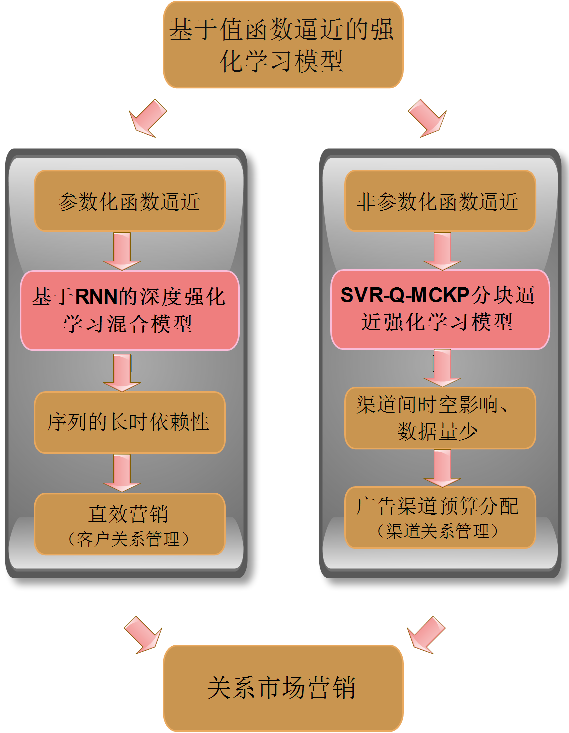
\includegraphics[width=0.5\textwidth]{研究路线}
\caption{本文研究路线}
\label{fig:研究内容}
\end{figure}

(1)在直效营销场景中,因为序列之间存在依赖性的影响,导致传统的深度强化学习不能较好的进行值函数的逼近。因此,本文提出了基于RNN的深度强化学习混合模型。该混合模型由两个网络构成,其中,利用RNN网络的长时依赖性可以从监督数据中较好的学习到观测信息的隐状态,然后将其作为状态输入,利用DQN网络强大的非线性逼近能力进行策略学习。两个网络协同控制与优化,可以在不需要借助专家领域知识的情况下,提高值函数的学习精度,以更好的实现直效营销场景中客户生命价值最大化的目标。与其它深度强化学习相比,该模型没有直接将环境的观测值作为强化学习的状态输入,而是将观测值的隐状态作为输入,并且为了进一步提高学习精度,通过改变网络结构,提出了一步混合模型和两步混合模型。

(2)在广告渠道预算分配场景中,因为存在数据量较少以及渠道间的时空影响等问题,导致传统的值函数逼近方法不能较好的进行值函数的学习。因此,本文提出了SVR-Q-MCKP分块逼近强化学习模型。其中,利用基于径向基核函数的SVR方法将强化学习中的值函数逼近转化为高维空间中的线性回归问题,以提高模型的学习速度;为了提高模型的逼近精度,提出了分块学习的强化学习思想。另外,通过考虑渠道之间的时空影响来重塑回报函数,并且通过改变行为探索的方法提高在小数据下探索的鲁棒性。最后,将带约束的预算分配问题与多选择背包问题相结合,输出最后的分配策略。

 (3)在实验验证阶段,将基于RNN的深度强化学习混合模型以及其它基准模型应用在直邮营销场景中,根据KDD-CUP-1998数据集进行模型训练,并且按照文献\citep{pednault2002sequential}中的方法构建仿真环境,比较、验证模型的效果。将基于DSP平台上的真实投放数据应用在SVR-Q-MCKP分块逼近强化学习模型中进行策略的学习与优化,并基于此数据构建仿真环境,最后在此仿真环境中比较、验证模型的效果。

\section{本文结构安排}
文本围绕强化学习技术在CRM领域中的部分应用展开研究,具体的组织结构如下:

第一章 绪论。首先介绍了本文的研究背景和选题意义,然后介绍了关系市场营销和强化学习的研究现状,主要包括本文所选择的直效营销和广告渠道资金分配两个领域的研究现状以及强化学习的发展历程、研究热点和发展趋势,接着阐明了本文的研究内容及贡献,最后介绍了本文的组织结构。

第二章 相关理论知识。
